\documentclass{beamer}
\usepackage[utf8]{inputenc}
\usepackage{cite}
\usetheme{Madrid}
\usecolortheme{default}
\usepackage{subcaption}


\title{Maximal Parking Lot Utilisation}
\author{Billy Jeremijenko, Yiwen Jiang, Joshua Morris}
\date{October 2021}

\AtBeginSection[]
{
  \begin{frame}
    \frametitle{Table of Contents}
    \tableofcontents[currentsection]
  \end{frame}
}
%------------------------------------------------------------


\begin{document}

%The next statement creates the title page.
\frame{\titlepage}


%---------------------------------------------------------
%This block of code is for the table of contents after
%the title page
\begin{frame}
\frametitle{Table of Contents}
\tableofcontents
\end{frame}
%---------------------------------------------------------


\section{Background}
\begin{frame}{The problem}
    Given a parking lot, we represent the parking lot as an $N \times M$ grid where each grid cell may have an obstacle.\medskip
    
    We require a model to find a layout, an allocation of parking and driving fields, which maximises the number of available parking spaces in the parking lot. 
\end{frame}

\begin{frame}{The problem}
    \begin{figure}
        \centering
        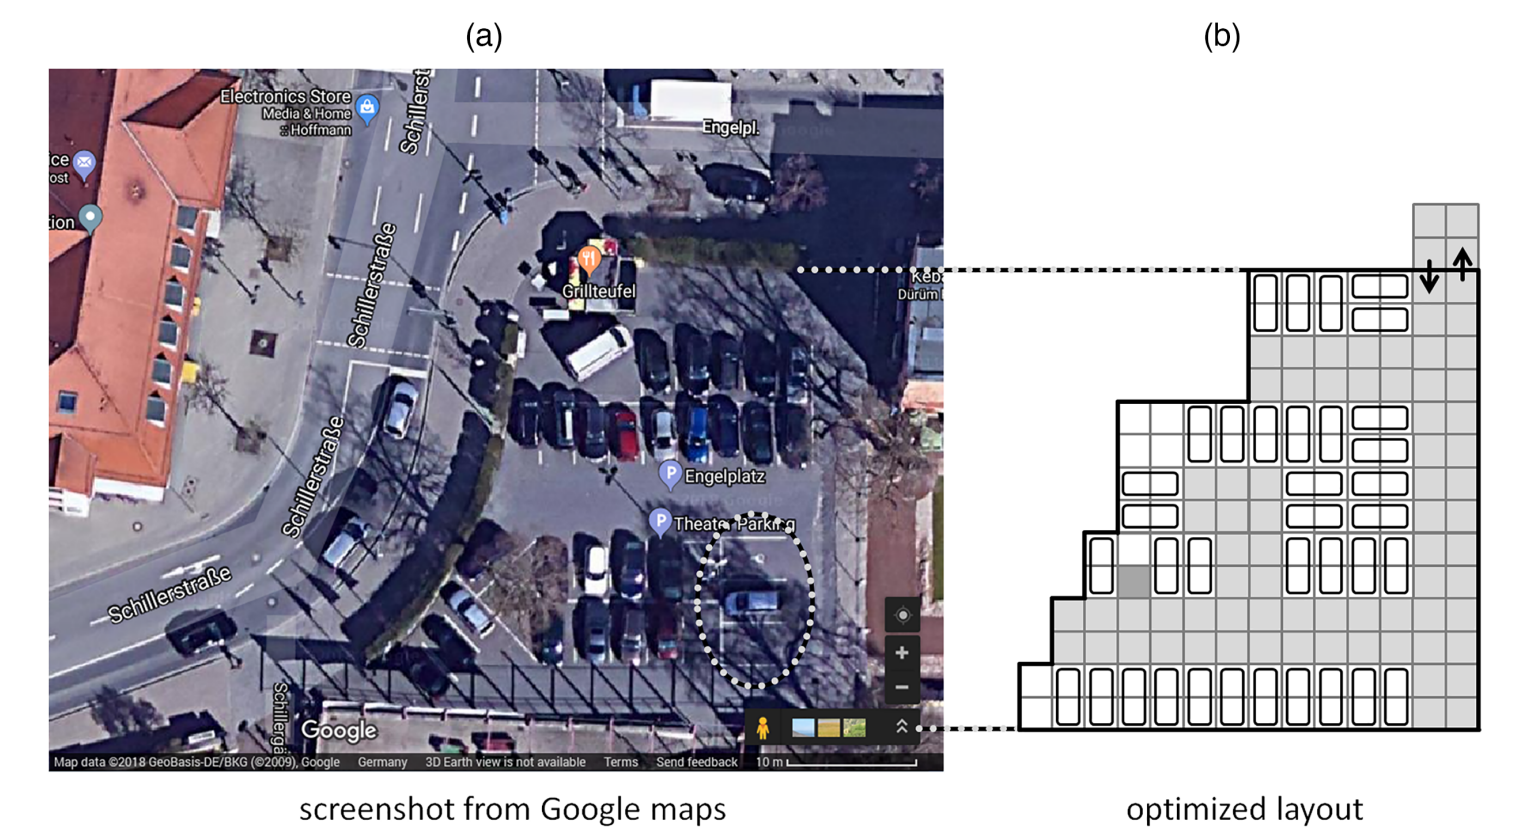
\includegraphics[width=0.7\textwidth]{figures/representation.PNG}
        \caption{An example of a parking lot begin represented by a grid\cite{paper}}
        \label{fig:fig}
    \end{figure}
\end{frame}

\begin{frame}{The paper}
    The paper\cite{paper} that we have built upon considers grid cells of varying resolutions. The $5m \times 5m$ grid cells allow for a simple formulation as each parking field and driving field is contained within one grid cell.\medskip
    
    However, at finer resolutions such as $2.5m \times 2.5m$ a parking space corresponds to two grid cells, which requires a more complex formulation, but allows for a closer to optimal solution.\medskip
    
    The flow model at a finer resolution has a large solution space due to directional variables and solved on an example $35m^2$ data set in $6$ hours. Our formulation solved on the same data in only $2$ minutes, and allows for arbitrarily fine grid cells.
\end{frame}

\section{Network flow formulation}

\begin{frame}{Sets and Data}
\textbf{Sets}\medskip

$S_1$ the set of grid cells on the border of the grid\medskip

$S_2$ the set of grid cells not on the border of the grid\medskip

$S = S_1 \cup S_2 = \{(i,j): i \in N,\, j \in M\}$ the set of grid cells\medskip

\textbf{Data}\medskip

$e$ the column of the entrance\medskip

$b_{ij} = 1$ if grid cell $(i,j) \in S$ is blocked\medskip

$M$ a big integer

\end{frame}

\begin{frame}{Variables}
\textbf{Variables}\medskip

$x_{ij} = 1$ if $(i, j) \in S$ is a parking field\medskip

$y_{ij} = 1$ if $(i, j) \in S$ is a driving field\medskip

$f_{ij}^\rightarrow \in \mathbb{R}$ horizontal flow from field $(i,j)$ to $(i,j+1)$ if $f_{ij}^\rightarrow > 0$, or from $(i,j+1)$ to $(i, j)$ otherwise\medskip

$f_{ij}^\downarrow \in \mathbb{R}$ vertical flow from field $(i,j)$ to $(i+1 , j)$ if $f_{ij}^\downarrow > 0$, or from $(i+1 , j)$ to $(i, j)$ otherwise
    
\end{frame}

\begin{frame}{Constraints}
\textbf{Constraints}\medskip

The entrance is accessible by a driving field
$$y_{0e} + y_{1e} = 2$$

In $S_1$ exactly one grid cell is enabled (the entrance, see previous constraint)
$$1 = \sum_{(i,j) \in S} (x_{ij} + y_{ij}) - \sum_{(i,j) \in S_2} (x_{ij} + y_{ij}) = 1$$

Parking fields are accessible by driving fields
$$x_{ij} \leq \sum_{(i', j') \in N(i, j)} y_{i'j'}, \, \forall (i,j) \in S$$

Each square serves at most a single purpose
$$x_{ij} + y_{ij} + b_{ij} \leq 1, \, \forall (i,j) \in S$$
\end{frame}

\begin{frame}{Flow Constraints}
\textbf{Flow Constraints}\medskip

Only driving fields send or receive flow
$$\lvert f_{ij}^\rightarrow \rvert \leq M \cdot y_{ij}, \, \forall (i,j) \in S$$
$$\lvert f_{ij}^\rightarrow \rvert \leq M \cdot y_{i(j+1)}, \, \forall (i,j) \in S$$
$$\lvert f_{ij}^\downarrow \rvert \leq M \cdot y_{ij}, \, \forall (i,j) \in S$$    
$$\lvert f_{ij}^\downarrow \rvert \leq M \cdot y_{(i+1)j}, \, \forall (i,j) \in S$$    

Every driving field has a net flow of at least one

$$y_{ij} \leq f_{ij}^\rightarrow + f_{ij}^\downarrow -f_{i(j+1)}^\rightarrow - f_{(i+1)j}^\downarrow,\, \forall (i,j) \in S_2$$

Net flow of driving fields does not exceed one
$$-f_{0e}^\downarrow \leq \sum_{(i,j) \in S_2} y_{ij}$$
\end{frame}

\begin{frame}{Objective}
\textbf{Objective}\medskip

Maximise the number of parking spaces, each parking field contains two

$$\textrm{maximize} \sum_{(i,j) \in S} 2 \cdot x_{ij}$$
    
\end{frame}

\begin{frame}{Network flow formulation}

    We omit the formulation at a finer resolution, which utilises multiple variables to represent the direction in which a parking lot is facing, due to time constraints.\medskip
    
    Furthermore, the model is slow to solve and made redundant by our own model which solves significantly faster. \medskip
    
    We have implemented the flow model at this finer resolution and the outcome is included it in our results.\medskip
    
    We now present our own solution focusing on the finer resolution.
\end{frame}

\section{Bender's decomposition and a priori column generation}
\begin{frame}{Bender's decomposition and a priori column generation}
\textbf{Our Solution}\medskip

The network flow model in the referenced paper is slow with larger grid sizes and finer resolutions.\medskip

It is also difficult to generalise to finer resolutions, requiring the introduction of multiple variables to indicate direction.\medskip

We develop a formulation based on a priori column generation to allow for various resolutions. As well as utilising lazy constraints, instead of flow constraints, to enforce the connectivity of driving fields.

\end{frame}

\begin{frame}{Sets and Data}
\textbf{Sets}

$S = \{(i,j): i \in N,\, j \in M\}$ the set of grid cells\medskip

$P$ the set of possible parking fields\medskip

$D$ the set of possible driving fields\medskip

\textit{$P$ and $D$ are generated a priori and consist of groups of $2 \times 1$ and $2 \times 2$ grid cells, respectively}

\medskip
\textbf{Data}

$p_{ijp} = 1$ if square $(i,j) \in S$ is contained in parking field $p \in P$\medskip

$d_{ijd} = 1$ if square $(i,j) \in S$ is contained in driving field $d \in D$\medskip

$b_{ij} = 1$ if square $(i,j) \in S$ is blocked\medskip

$e$ the driving field $d\in D$ corresponding to the entrance and exit
\end{frame}

\begin{frame}{Variables}
\textbf{Variables}\medskip

$x_p = 1$ if parking field $p\in P$ is enabled\medskip

$y_d = 1$ if driving field $d \in D$ is enabled
    
\end{frame}

\begin{frame}{Constraints}
\textbf{Constraints}\medskip

The entrance and exit are accessible by a driving field
$$y_e = 1$$\medskip

Parking fields do not share grid cells
$$\sum_{p \in P} p_{ijp}\cdot x_p \leq 1,\, \forall(i,j) \in S$$\medskip

Parking fields are adjacent to a driving field
$$x_p \leq \sum_{d \in N(p)} y_d, \, \forall p\in P$$
\end{frame}

\begin{frame}{Constraints}
\textbf{Constraints}\medskip

Each grid cell serves at most a single purpose
$$\sum_{p \in P} p_{ijp} \cdot x_p + \sum_{d \in D} \frac{1}{4} \cdot d_{ijd} \cdot y_d + b_{ij} \leq 1,\, \forall(i,j) \in S$$\medskip

Each driving field is adjacent to a driving field
$$y_d \leq \sum_{d' \in N(d)} y_{d'},\, \forall d \in D$$
\end{frame}

\begin{frame}{Objective}
\textbf{Objective}\medskip

Maximise the number of parking fields, that is
$$\textrm{maximise} \sum_{p \in P} x_p$$
    
\end{frame}

\begin{frame}{Lazy Constraints}
\textbf{Lazy Constraints}\medskip

This formulation allows for a solution which has multiple contiguous regions of driving fields which are disconnected from each other, resulting in a solution in which parking fields are not accessible from the entrance. \medskip

Given an optimal solution $y_i$ to the master problem with disconnected regions $\mathcal{C} = C_1 \cup C_2 \cup \cdots \cup C_k$ add the following constraint
$$y_d \leq \sum_{d' \in N(C)} y_d, \, \forall C \in \mathcal{C}, \, \forall d \in D$$
    
\end{frame}

\section{Results}
\begin{frame}{Results}
    We run our models on the same data as used for demonstration purposes in the paper, which was based on real world data. For the finer grid cells, our model solves in 1.87 minutes which is faster than the 5.96 hour solve time of the paper.

    \begin{table}[]
        \centering
        \begin{tabular}{c|c|c}
           Model  & Time (s) & Iterations \\
             \hline
            R1 Flow &    4.81  & 22 \\
            R1 Lazy &  0.32 & 13 \\
            R2 Flow &    21458.08  & 2672 \\
            R2 Lazy &  112.97 & 58 
        \end{tabular}
        \caption{Results for Models from Paper and Lazy Constraints}
        \label{tab:my_label}
    \end{table}
\end{frame}

\begin{frame}{Resolution One Optimal Solution}

    The optimal solution for resolution one fits 38 parking spaces
    \begin{figure}
        \centering
        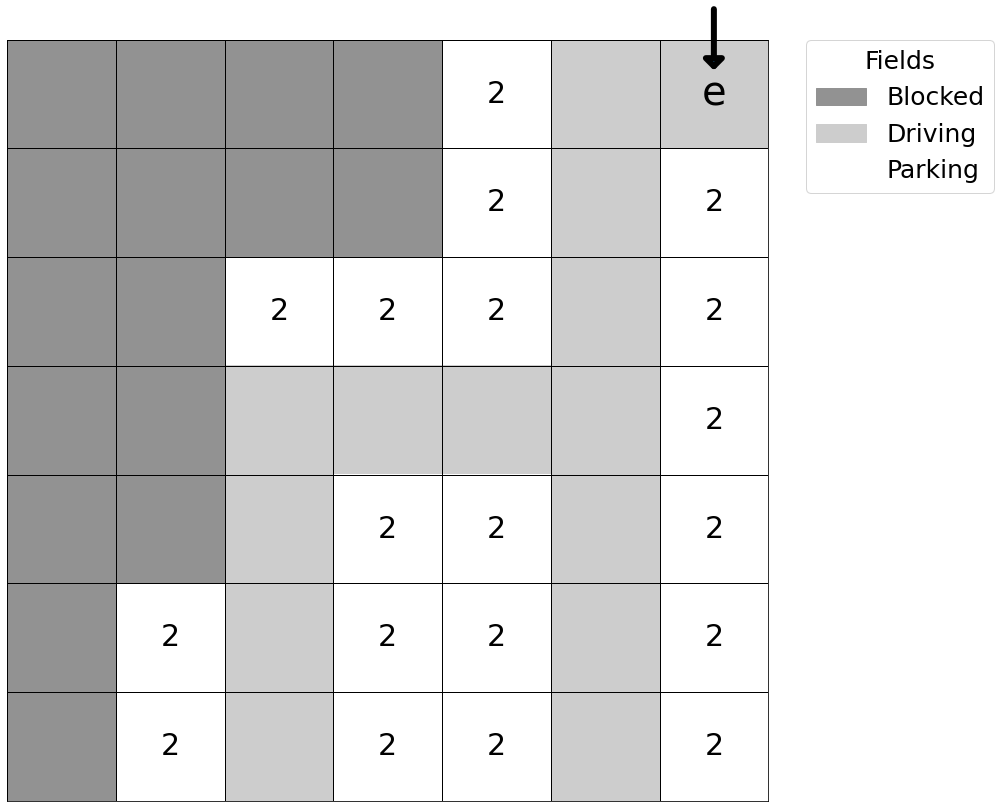
\includegraphics[width=0.6\textwidth]{figures/solution_r1lazy.png}
        \caption{Optimal layout for resolution one}
        \label{fig:fig}
    \end{figure}
\end{frame}

\begin{frame}{Resolution Two Optimal Solution}

    The optimal solution for resolution two fits 40 parking spaces

    \begin{figure}
        \centering
        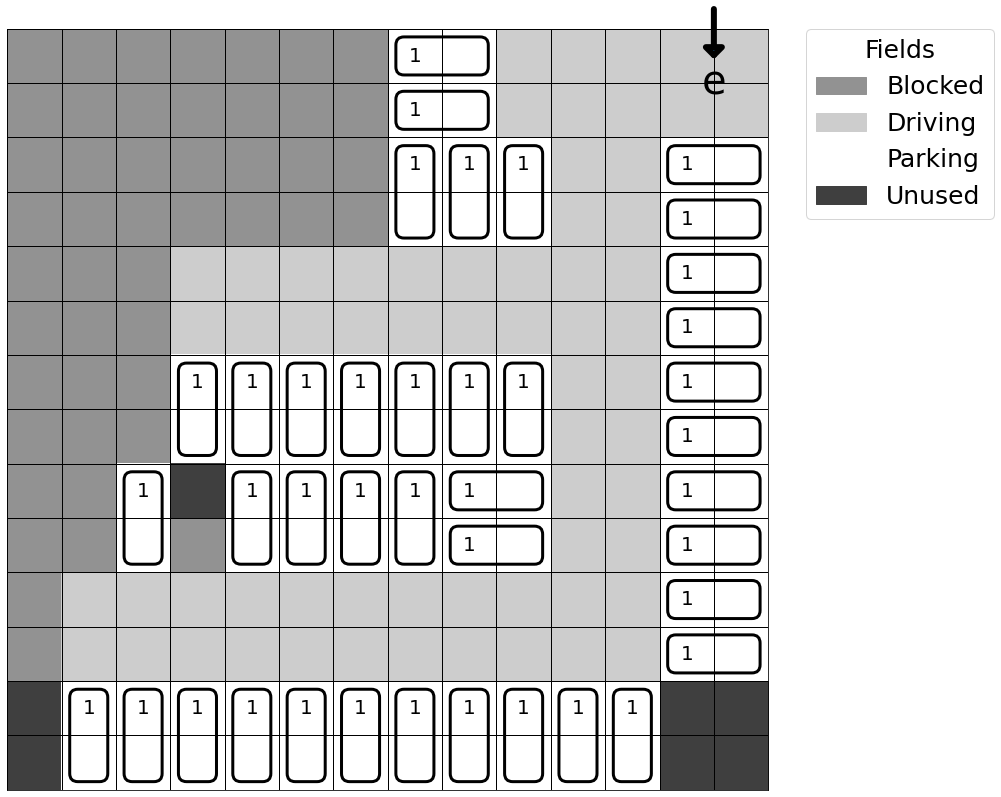
\includegraphics[width=0.6\textwidth]{figures/solution_r2lazy.png}
        \caption{Optimal layout for resolution two}
        \label{fig:fig}
    \end{figure}
\end{frame}

\begin{frame}{Coarse Resolution Evolution}
    \begin{figure}
    \begin{subfigure}{.5\textwidth}
      \centering
      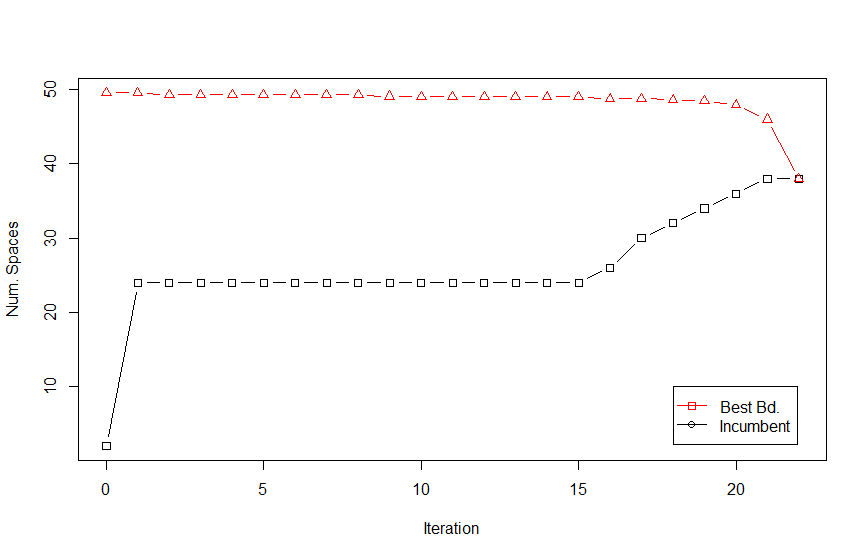
\includegraphics[width=1\linewidth]{figures/res1paper.png}
      \caption{Network Flow}
      \label{fig:sfig1}
    \end{subfigure}%
    \begin{subfigure}{.5\textwidth}
      \centering
      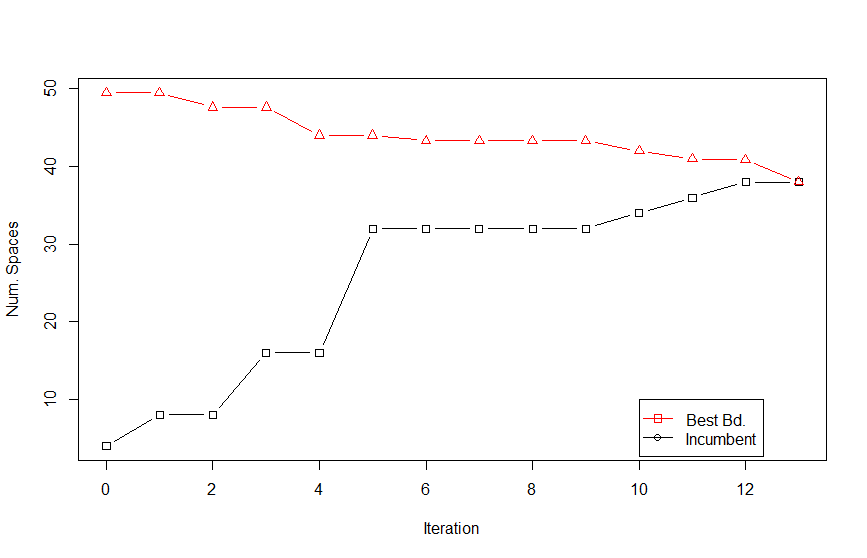
\includegraphics[width=1\linewidth]{figures/res1lazy.png}
      \caption{Lazy Constraints}
      \label{fig:sfig2}
    \end{subfigure}
    \caption{Evolution of resolution one models}
    \label{fig:fig}
    \end{figure}
\end{frame}

\begin{frame}{Fine Resolution Evolution}
    \begin{figure}
    \begin{subfigure}{.5\textwidth}
      \centering
      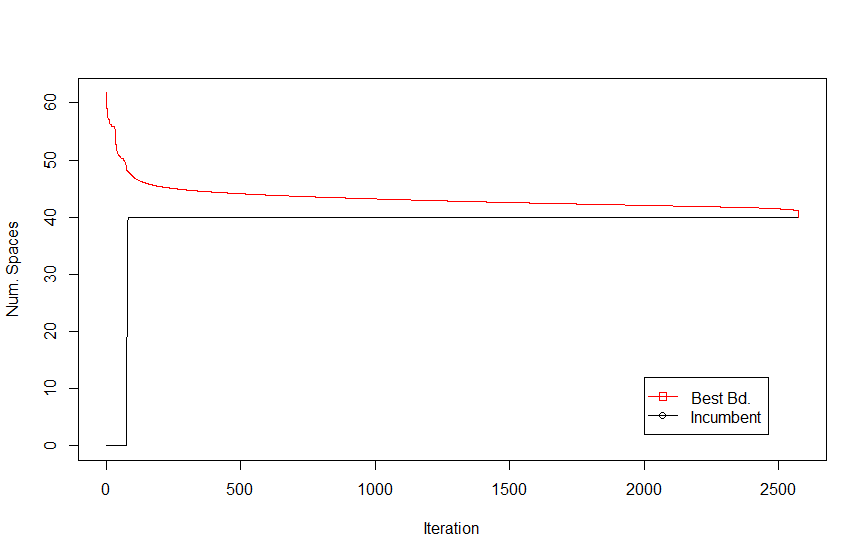
\includegraphics[width=1\linewidth]{figures/res2paper.png}
      \caption{Network Flow}
      \label{fig:sfig1}
    \end{subfigure}%
    \begin{subfigure}{.5\textwidth}
      \centering
      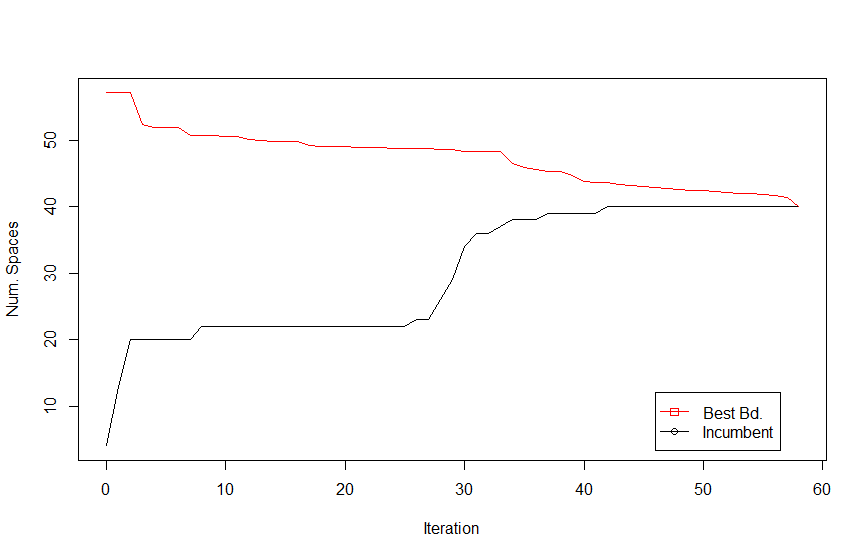
\includegraphics[width=1\linewidth]{figures/res2lazy.png}
      \caption{Lazy Constraints}
      \label{fig:sfig2}
    \end{subfigure}
    \caption{Evolution of resolution two models}
    \label{fig:fig}
    \end{figure}
\end{frame}

\begin{frame}{Bibliography}
    \bibliographystyle{amsalpha}
    \bibliography{ref.bib}
\end{frame}
\end{document}